\documentclass[10pt,a4paper]{article}

\usepackage[a4paper,margin=0.75in]{geometry}
\usepackage[T1]{fontenc}
\usepackage[utf8]{inputenc}
\usepackage[english]{babel}
\usepackage{lmodern}
\usepackage{microtype}
\usepackage{amsmath,amssymb}
\usepackage{booktabs}
\usepackage{hyperref}
\usepackage{enumitem}
\usepackage{float}
\usepackage{placeins}
\usepackage{pgfplots}
\usepackage{xcolor}

\pgfplotsset{compat=1.18}

\hypersetup{
  colorlinks=true,
  linkcolor=blue!50!black,
  urlcolor=blue!50!black,
  citecolor=blue!50!black
}

\setlength{\parindent}{0pt}
\setlength{\parskip}{0.35em}
\setlist{nosep,leftmargin=*}

% Set \anonymoustrue before preparing an anonymous submission.
\newif\ifanonymous
\anonymoustrue

\newcommand{\oldAInitWin}{0.008}
\newcommand{\oldBInitWin}{0.084}
\newcommand{\oldInitTie}{0.908}
\newcommand{\oldABTrainedWin}{0.492}
\newcommand{\oldTrainedAWin}{0.506}
\newcommand{\oldTrainedBWin}{0.006}
\newcommand{\oldAAgainstInitB}{0.916}
\newcommand{\oldAInitReward}{0.0026}
\newcommand{\oldBInitReward}{0.0084}
\newcommand{\oldBTrainedReward}{0.0548}
\newcommand{\oldATrainedReward}{0.1000}
\newcommand{\newAWinEightHundred}{0.324}
\newcommand{\newBWinEightHundred}{0.517}
\newcommand{\newTieEightHundred}{0.159}
\newcommand{\newARewardEightHundred}{0.1429}
\newcommand{\newBRewardEightHundred}{0.1714}
\newcommand{\newAWinThousand}{0.340}
\newcommand{\newBWinThousand}{0.516}
\newcommand{\newTieThousand}{0.143}
\newcommand{\newARewardThousand}{0.1429}
\newcommand{\newBRewardThousand}{0.1721}

\title{\vspace{-1em}Toward Multi-Agent Nash Learning from Human Feedback: \\ Heterogeneous Cross-Play in VERL}
\ifanonymous
  \author{}
\else
  \author{Vasiagina Ekaterina \and Ignashin Igor}
\fi
\date{}

\begin{document}
\maketitle
\vspace{-1.4em}

\begin{abstract}
Nash Learning from Human Feedback (NLHF) formulates alignment through pairwise preferences and game dynamics rather than through a single scalar reward model \cite{nlhf}. The original formulation considers competition against previous versions of the same policy. This work studies a multi-model variant in which different live models compete online. A heterogeneous \textit{CrossPlay} recipe is implemented in VERL: two instruction-tuned LLMs answer the same prompt, an external judge compares their outputs, and both policies are updated through DPO-style preference pairs. The first experiment showed strong but potentially biased one-sided improvement under a coarse rule-based judge and failure-only replay. A revised version increased the response budget from 24 to 128 tokens, introduced a denser GSM8K reward, and equalized replay examples, DPO pairs, and update steps across both policies. On full GSM8K validation, checkpoints 800 and 1000 show a non-degenerate matchup: policy $B$ remains stronger, while policy $A$ improves from 0.324 to 0.340 win rate.
\end{abstract}

\textbf{Motivation and task.}
NLHF is attractive because pairwise preferences can represent comparison-dependent or non-transitive feedback more naturally than a single scalar reward. However, the original setup mainly compares a policy with past versions of itself. This work studies a more direct multi-agent variant: two different model families are trained in the same loop and learn from pairwise comparisons on the same prompts. The goal is to build and evaluate a working experimental setup for heterogeneous preference-based training.

\textbf{Relation to NLHF.}
In NLHF, a prompt $x$ and two responses $(y_a,y_b)$ are evaluated by a preference model
\[
P_\phi(y_a \succ y_b \mid x),
\]
and learning is formulated as a game against a competing policy \cite{nlhf}. In the current approximation, two policies $\pi_A$ and $\pi_B$ generate
\[
y_A \sim \pi_A(\cdot \mid x), \qquad y_B \sim \pi_B(\cdot \mid x),
\]
after which an external judge forms a chosen/rejected pair for the losing side. This differs from the original NLHF formulation in two ways: the judge is not a learned pairwise preference model, and the update remains DPO-style rather than a direct Nash optimization step. However, the setup is already substantially closer to the intended multi-agent game than single-policy self-play against historical samples.
Thus, the implemented algorithm should be viewed as an intermediate point between standard DPO-style preference optimization and full NLHF: it keeps the live-opponent training loop, but still derives preferences from a verifiable task judge.

\textbf{Implementation.}
The main artifact is a new \texttt{crossplay} pipeline in VERL. For each prompt $x$, two policies generate responses $y_A \sim \pi_A(\cdot|x)$ and $y_B \sim \pi_B(\cdot|x)$; a judge returns scores $s_A$ and $s_B$. If $s_A > s_B$, then $(y_A,y_B)$ becomes the chosen/rejected pair, and the reverse pair is used when $s_B > s_A$. Each policy is updated against its own frozen anchor $\rho$ using a DPO-style logit
\[
z_\pi(x,y^+,y^-)
=
\beta\big[(\log\pi(y^+|x)-\log\pi(y^-|x))-(\log\rho(y^+|x)-\log\rho(y^-|x))\big].
\]
Different tokenizers are handled by retokenizing both textual responses under the policy being updated; the same pipeline also supports replay buffers, checkpoint save/resume, and offline checkpoint matchups.

\textbf{Experiments.}

\textit{Initial cross-play setting.}
\newline
The first stable experiment used $\texttt{Qwen2.5-0.5B-Instruct}$ as policy $A$ and $\texttt{SmolLM2-1.7B-Instruct}$ as policy $B$ on GSM8K \cite{gsm8k}. Training used a short response budget of 24 generated tokens, a rule-based GSM8K judge (\texttt{crossplay\_gsm8k\_rule}), and failure-only replay. The judge assigned reward 1.0 to exact final-answer matches, 0.1 to parseable but incorrect answers, and 0.0 when no valid final answer was extracted. Offline validation on a 500-example prefix is summarized in Figure~\ref{fig:legacy-results}. The larger model was initially stronger, but after training the smaller model appeared to improve substantially. These results showed that the pipeline can drive strong behavioral change. At the same time, they also exposed a likely source of bias: the combination of a coarse judge, a very short reasoning budget, and failure-only replay can create an apparent one-sided advantage by giving one policy more useful update examples.

\begin{figure}[h]
\centering
\begin{minipage}[t]{0.48\linewidth}
\centering
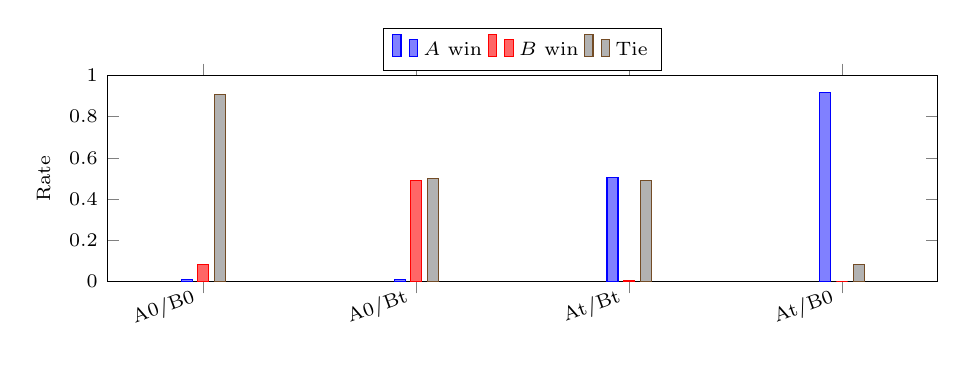
\begin{tikzpicture}
\begin{axis}[
  width=\linewidth,
  height=4.2cm,
  ybar,
  bar width=4pt,
  ymin=0,
  ymax=1.0,
  symbolic x coords={A0/B0,A0/Bt,At/Bt,At/B0},
  xtick=data,
  xticklabel style={font=\scriptsize,rotate=20,anchor=east},
  yticklabel style={font=\scriptsize},
  ylabel={Rate},
  ylabel style={font=\scriptsize},
  legend style={font=\scriptsize,at={(0.5,1.02)},anchor=south,legend columns=3},
  enlarge x limits=0.15
]
\addplot+[fill=blue!50] coordinates {
  (A0/B0,\oldAInitWin)
  (A0/Bt,0.008)
  (At/Bt,\oldTrainedAWin)
  (At/B0,\oldAAgainstInitB)
};
\addplot+[fill=red!60] coordinates {
  (A0/B0,\oldBInitWin)
  (A0/Bt,\oldABTrainedWin)
  (At/Bt,\oldTrainedBWin)
  (At/B0,0.000)
};
\addplot+[fill=gray!60] coordinates {
  (A0/B0,\oldInitTie)
  (A0/Bt,0.500)
  (At/Bt,0.488)
  (At/B0,0.084)
};
\legend{$A$ win,$B$ win,Tie}
\end{axis}
\end{tikzpicture}
\end{minipage}\hfill
\begin{minipage}[t]{0.48\linewidth}
\centering
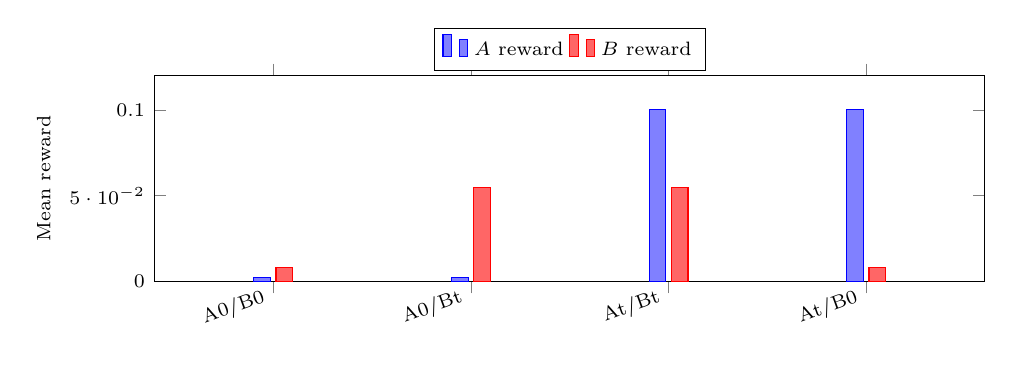
\begin{tikzpicture}
\begin{axis}[
  width=\linewidth,
  height=4.2cm,
  ybar,
  bar width=6pt,
  ymin=0,
  ymax=0.12,
  symbolic x coords={A0/B0,A0/Bt,At/Bt,At/B0},
  xtick=data,
  xticklabel style={font=\scriptsize,rotate=20,anchor=east},
  yticklabel style={font=\scriptsize},
  ylabel={Mean reward},
  ylabel style={font=\scriptsize},
  legend style={font=\scriptsize,at={(0.5,1.02)},anchor=south,legend columns=2},
  enlarge x limits=0.20
]
\addplot+[fill=blue!50] coordinates {
  (A0/B0,\oldAInitReward)
  (A0/Bt,\oldAInitReward)
  (At/Bt,\oldATrainedReward)
  (At/B0,\oldATrainedReward)
};
\addplot+[fill=red!60] coordinates {
  (A0/B0,\oldBInitReward)
  (A0/Bt,\oldBTrainedReward)
  (At/Bt,\oldBTrainedReward)
  (At/B0,\oldBInitReward)
};
\legend{$A$ reward,$B$ reward}
\end{axis}
\end{tikzpicture}
\end{minipage}
\caption{Cross-play validation results on a 500-example prefix. Left: win/tie rates. Right: mean rule-judge rewards. Here $A_0$ and $B_0$ denote initial policies, while $A_t$ and $B_t$ denote trained policies from the legacy run.}
\label{fig:legacy-results}
\end{figure}

\textit{Improved cross-play setting.}\newline
The revised run modifies three parts of the pipeline. First, the response budget is increased to 128 tokens to allow short reasoning traces. Second, the reward is replaced by a denser GSM8K signal with a canonical final-answer format \texttt{\#\#\#\# <answer>}. The dense reward keeps exact final-answer correctness as the main signal, but adds small shaping terms for parseable final answers and numeric proximity, with incorrect answers capped below exact matches. Third, update imbalance is explicitly removed: replay examples, selected DPO pairs, and update counts are logged and equalized for both models.

\textit{Current run and checkpoint evaluation.}
The revised run again uses Qwen-0.5B vs.\ SmolLM2-1.7B on GSM8K, but with a 2000-example training subset, 128-token responses, dense reward, and balanced all-pair updates. The key quantitative property of the run is exact balance of training opportunities:
\[
\Delta_{\text{replay}} = \Delta_{\text{pairs}} = \Delta_{\text{updates}} = 0.
\]
In contrast to the earlier one-sided pattern, the online metrics become oscillatory: on mid-run segments, $A$-wins, $B$-wins, and ties all occur. This suggests that the revised setup behaves more like a genuine competition and less like a process dominated by unequal update exposure. Full validation was completed for checkpoints 800 and 1000; the corresponding results are shown in Table~\ref{tab:newval} and Figure~\ref{fig:new-results}. Compared with the legacy $A_t$ vs.\ $B_t$ result, where $A$ dominated with 0.506 win rate against 0.006 for $B$, the revised evaluation is more balanced: at checkpoint 1000, $A$ reaches 0.340 while $B$ remains ahead at 0.516.

\begin{table}[H]
\centering
\scriptsize
\begin{minipage}[t]{0.46\linewidth}
\centering
\begin{tabular}{@{}ll@{}}
\toprule
Setting & Value \\
\midrule
Train subset & 2000 GSM8K \\
Response budget & 128 tokens \\
Reward & dense GSM8K \\
Update accounting & balanced \\
Saved ckpts & 200--1200 \\
Stopped at & 1357 / 2000 \\
Validation & ckpt 800, 1000 \\
\bottomrule
\end{tabular}
\end{minipage}\hfill
\begin{minipage}[t]{0.50\linewidth}
\centering
\begin{tabular}{@{}lccccc@{}}
\toprule
Ckpt & $A$ win & $B$ win & Tie & $A$ r. & $B$ r. \\
\midrule
800  & \newAWinEightHundred & \newBWinEightHundred & \newTieEightHundred & \newARewardEightHundred & \newBRewardEightHundred \\
1000 & \newAWinThousand     & \newBWinThousand     & \newTieThousand     & \newARewardThousand     & \newBRewardThousand \\
\bottomrule
\end{tabular}
\end{minipage}
\caption{Revised run configuration and full-validation results on GSM8K.}
\label{tab:newval}
\end{table}

\begin{figure}[H]
\centering
\begin{minipage}[t]{0.48\linewidth}
\centering
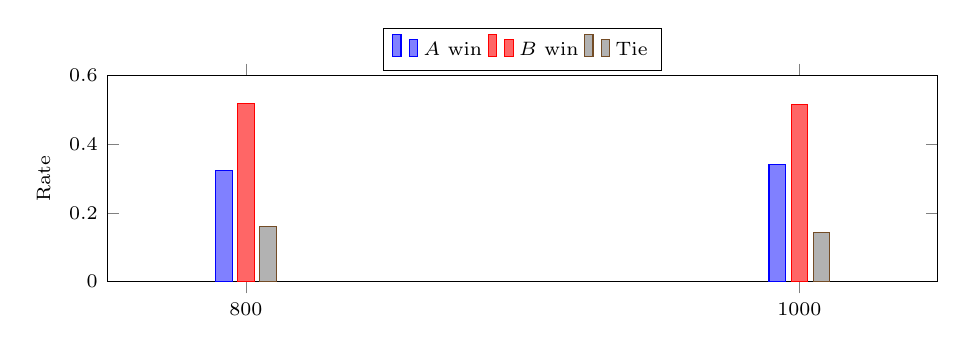
\begin{tikzpicture}
\begin{axis}[
  width=\linewidth,
  height=4.2cm,
  ybar,
  bar width=6pt,
  ymin=0,
  ymax=0.60,
  symbolic x coords={800,1000},
  xtick=data,
  xticklabel style={font=\scriptsize},
  yticklabel style={font=\scriptsize},
  ylabel={Rate},
  ylabel style={font=\scriptsize},
  legend style={font=\scriptsize,at={(0.5,1.02)},anchor=south,legend columns=3},
  enlarge x limits=0.25
]
\addplot+[fill=blue!50] coordinates {
  (800,\newAWinEightHundred)
  (1000,\newAWinThousand)
};
\addplot+[fill=red!60] coordinates {
  (800,\newBWinEightHundred)
  (1000,\newBWinThousand)
};
\addplot+[fill=gray!60] coordinates {
  (800,\newTieEightHundred)
  (1000,\newTieThousand)
};
\legend{$A$ win,$B$ win,Tie}
\end{axis}
\end{tikzpicture}
\end{minipage}\hfill
\begin{minipage}[t]{0.48\linewidth}
\centering
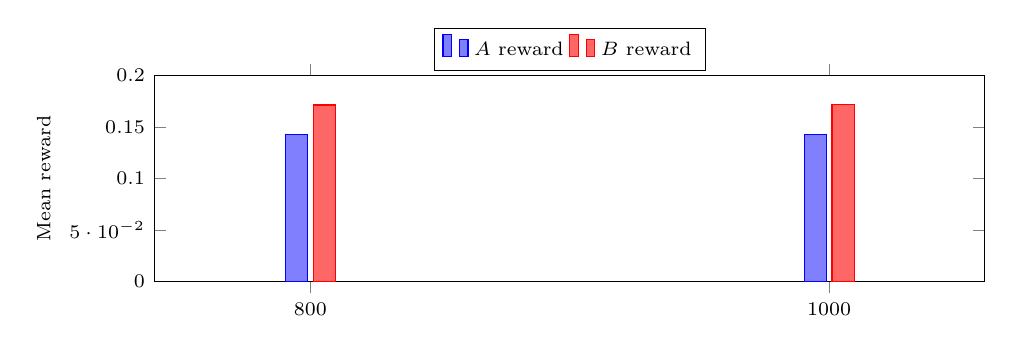
\begin{tikzpicture}
\begin{axis}[
  width=\linewidth,
  height=4.2cm,
  ybar,
  bar width=8pt,
  ymin=0,
  ymax=0.20,
  symbolic x coords={800,1000},
  xtick=data,
  xticklabel style={font=\scriptsize},
  yticklabel style={font=\scriptsize},
  ylabel={Mean reward},
  ylabel style={font=\scriptsize},
  legend style={font=\scriptsize,at={(0.5,1.02)},anchor=south,legend columns=2},
  enlarge x limits=0.30
]
\addplot+[fill=blue!50] coordinates {
  (800,\newARewardEightHundred)
  (1000,\newARewardThousand)
};
\addplot+[fill=red!60] coordinates {
  (800,\newBRewardEightHundred)
  (1000,\newBRewardThousand)
};
\legend{$A$ reward,$B$ reward}
\end{axis}
\end{tikzpicture}
\end{minipage}
\caption{Full-validation results for the revised balanced run. Left: win/tie rates at checkpoints 800 and 1000. Right: mean dense-judge rewards at the same checkpoints.}
\label{fig:new-results}
\end{figure}

\textbf{Interpretation.}
The revised result should not be interpreted as final mathematical reasoning improvement. Rather, it shows that the earlier large advantage of policy $A$ was not robust to a better-controlled training regime. After balancing the number of update examples, the larger SmolLM2-1.7B policy remains stronger on full validation, while Qwen2.5-0.5B still improves during training. This is a useful outcome for the project: it separates a real competitive training signal from an artifact of unequal replay exposure. An important limitation remains explicit: the current system still uses a scalar/dense judge rather than a learned pairwise preference model in the sense of NLHF.

\textbf{Conclusion.}
The completed part of the project is a working heterogeneous cross-play training and evaluation setup. The current experiments indicate that update accounting and reward design materially affect the observed game dynamics. The next methodological step is to replace the scalar GSM8K judge with a learned pairwise preference model, which would move the setup closer to NLHF and allow direct study of non-transitive preferences.

\FloatBarrier
\begin{thebibliography}{9}

\bibitem{nlhf}
R.~Munos, M.~Valko, D.~Calandriello, M.~Gheshlaghi Azar, M.~Rowland, Z.~D.~Guo, Y.~Tang, M.~Geist, T.~Mesnard, A.~Michi, M.~Selvi, S.~Girgin, N.~Momchev, O.~Bachem, D.~J.~Mankowitz, D.~Precup, and B.~Piot.
\newblock Nash Learning from Human Feedback.
\newblock \emph{arXiv preprint arXiv:2312.00886}, 2024.

\bibitem{gsm8k}
K.~Cobbe, V.~Kosaraju, M.~Bavarian, M.~Chen, H.~Jun, L.~Kaiser, M.~Plappert, J.~Tworek, J.~Hilton, R.~Nakano, C.~Hesse, and J.~Schulman.
\newblock Training Verifiers to Solve Math Word Problems.
\newblock \emph{arXiv preprint arXiv:2110.14168}, 2021.

\bibitem{dpo}
R.~Rafailov, A.~Sharma, E.~Mitchell, C.~D.~Manning, S.~Ermon, and C.~Finn.
\newblock Direct Preference Optimization: Your Language Model Is Secretly a Reward Model.
\newblock \emph{Advances in Neural Information Processing Systems}, 36, 2023.

\end{thebibliography}

\end{document}
